\documentclass[12pt]{article}

\usepackage[T2A]{fontenc}
\usepackage[utf8]{inputenc}
\usepackage[english, russian]{babel}
\usepackage[sups]{XCharter}
\usepackage[vvarbb, uprightscript, charter, scaled=1.05]{newtxmath}
\usepackage{enumitem}
\usepackage{verbatim}
\usepackage[justification=centering]{caption}
% \usepackage{caption}
% \captionsetup[figure]{skip=1pt}
\usepackage{microtype}
\usepackage{subcaption}
% \usepackage[style=numeric, sorting=none]{biblatex}
% \addbibresource{refs.bib}
% \usepackage{minted}
% \usepackage{fancyhdr}
% \usepackage{gensymb}
% \usepackage{booktabs}
% \usepackage{ntheorem}
% \usepackage{mathtools}
\usepackage{geometry}
% \usepackage{titling}  
\usepackage{indentfirst}
% \usepackage[normalem]{ulem}
% \useunder{\uline}{\ul}{}
\usepackage{graphicx}
\graphicspath{ {vis/} }

\usepackage[table,xcdraw]{xcolor}
\usepackage{hyperref}
\hypersetup{
    colorlinks=true,
    linkcolor=blue,
    filecolor=magenta,      
    urlcolor=cyan,
}

\geometry{a4paper, textwidth=16cm, textheight=24cm}

\newcommand{\mpl}[2]{
    \begin{figure}[!h]
        \includegraphics[width=0.98\textwidth]{#1}
        \centering
        \caption{#2}
        \label{fig:#1}
     \end{figure}
}

\title{Отчет по лабораторной работе №1\break
\normalsize курса <<Обработка и распознавание изображений>>
}

\author{Васильев Руслан \and{ВМК МГУ, 317 группа}}

\usepackage{tocloft}
\renewcommand{\cftsecleader}{\cftdotfill{\cftdotsep}}

\begin{document}

\maketitle
\tableofcontents
\newpage
\setcounter{secnumdepth}{0}

\section{Постановка задачи}
Цель лабораторной работы~--- написать программу для работы с фишками настольной игры <<тримино>>. Этапы работы программы:
\begin{enumerate}
    \item Считывание входных изображений;
    \item Обработку изображений, в которую входят:
    \begin{itemize}
        \item Сегментация игровых фишек,
        \item Подсчет точек, соответствующих вершинам найденных фишек;
    \end{itemize}
    \item Вывод в файл координат центров фишек и количества точек в углах;
    \item Отображение на экране наглядного изображения, иллюстрирующего сегментацию и подсчет точек.
\end{enumerate}

Кроме того, программа задумывается не только как <<черный ящик>>, но и модуль, из которого можно импортировать функции и настраивать их параметры, улучшая качество сегментации и точность подсчета точек.

\section{Описание данных}

Данные, подающиеся на вход,~--- фотографии фишек, хранящиеся в формате BMP24. Таким образом, мы работаем с трехканальными изображениями, где глубина каждого цвета~--- 8 бит. Примеры, предложенные в задании, изображены на \autoref{fig:input}.

\begin{figure}[!h]
    \begin{subfigure}{.32\linewidth}
    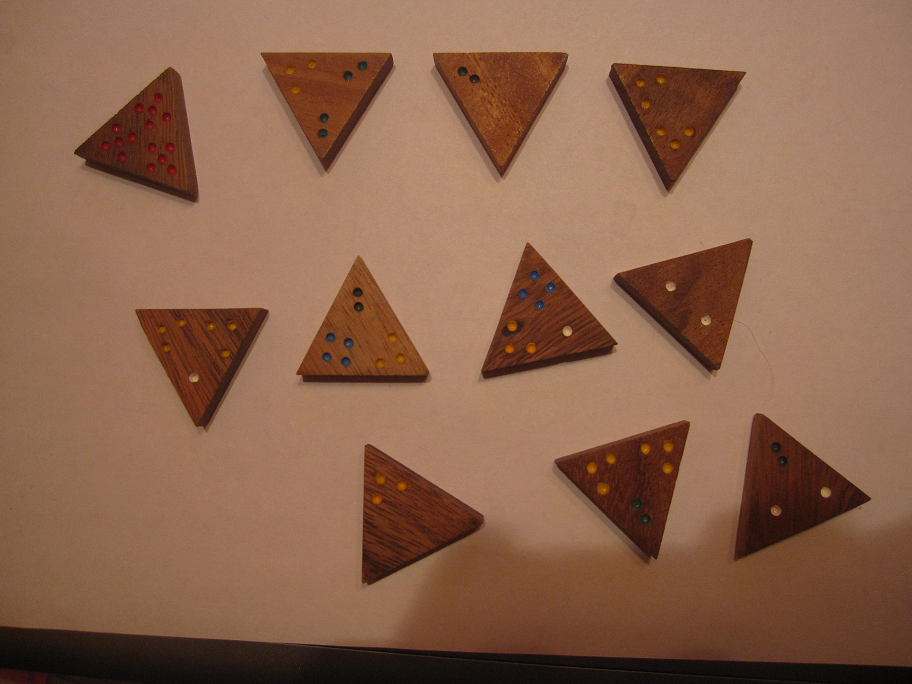
\includegraphics[width=0.93\linewidth]{Pict_1_1.png}
    \centering
    \caption{Beginner, Pict\_1\_1}
    \label{fig:input_beginner}
    \end{subfigure}
    \begin{subfigure}{.32\linewidth}
    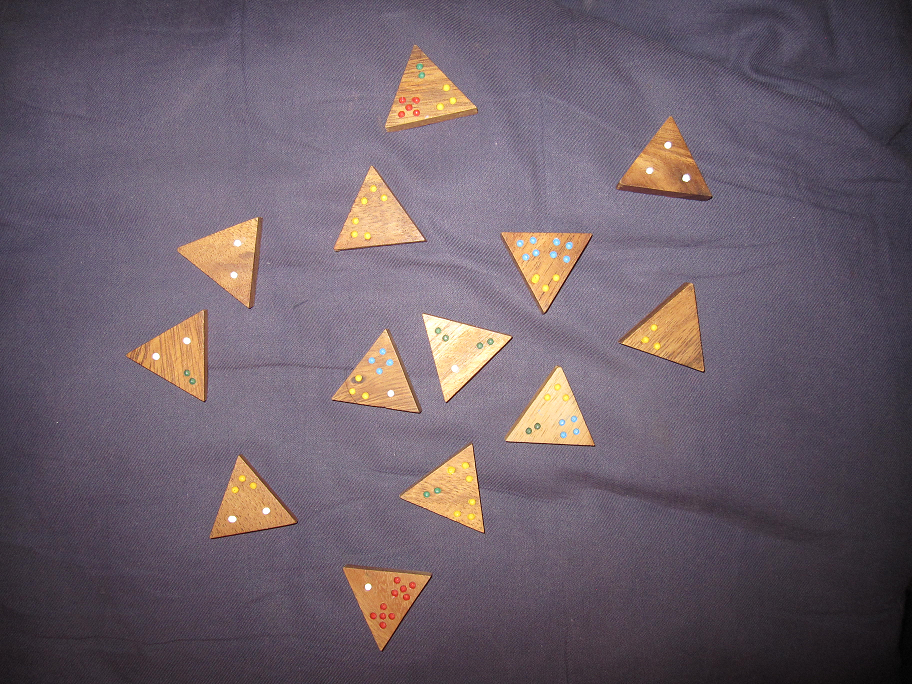
\includegraphics[width=0.93\linewidth]{Pict_2_1.png}
    \centering
    \caption{Intermediate, Pict\_2\_1}
    \label{fig:input_intermediate}
    \end{subfigure}
    \begin{subfigure}{.32\linewidth}
    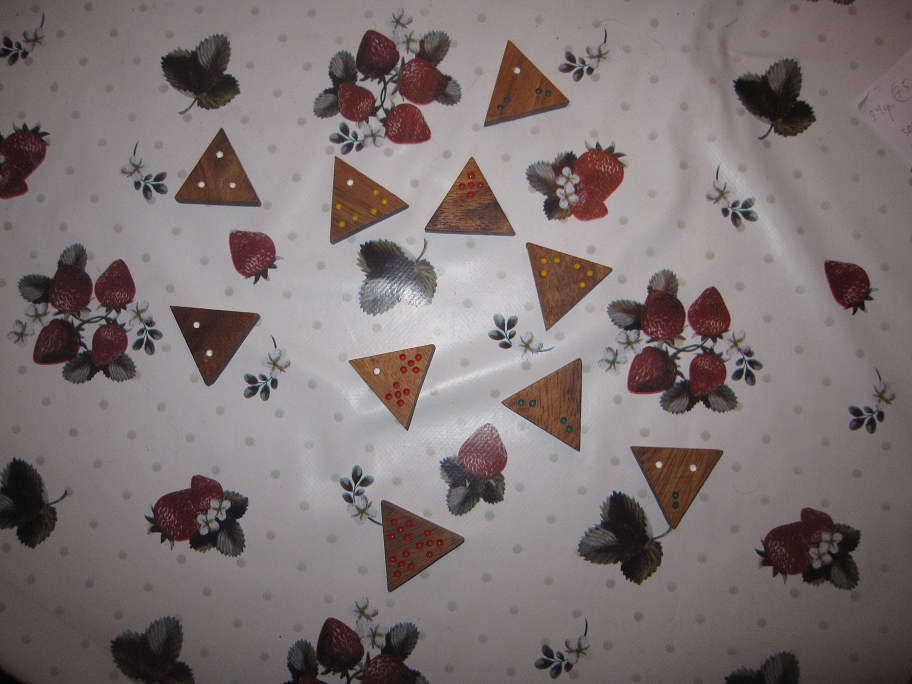
\includegraphics[width=0.93\linewidth]{Pict_4_1.png}
    \centering
    \caption{Expert, Pict\_4\_1}
    \label{fig:input_expert}
    \end{subfigure}
    \centering
    \caption{Примеры входных изображений}
    \label{fig:input}
\end{figure}

Три уровня сложности связаны с фоном и освещенностью. В простейшем случае изображение имеет гладкий фон и однородное освещение, в худшем на фоне расположены дополнительные элементы, а фишки освещены неравномерно. От решения требуется устойчивость к таким особенностям.

\section{Метод решения}
Решение разделяется на два ключевых этапа: сегментация фишек и поиск точек внутри найденных объектов. На каждом этапе совершается последовательность из нескольких преобразований изображения, которую мы продемонстрируем на вырезанном фрагменте из <<сложного>> уровня (\verb|Pict_3_1.bmp|), \autoref{fig:fragment_input}. Оставим также координатную сетку для наглядности.

\begin{figure}[!h]
    \begin{subfigure}{.45\linewidth}
        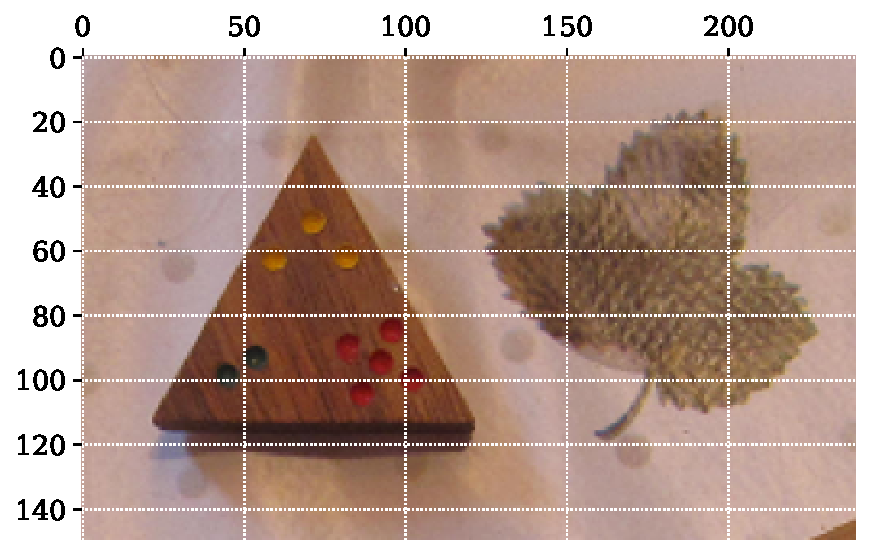
\includegraphics[width=.93\linewidth]{fragment_input.pdf}
        \centering
        \caption{Фрагмент Pict\_3\_1.bmp}
        \label{fig:fragment_input}
    \end{subfigure}
    \begin{subfigure}{.45\linewidth}
        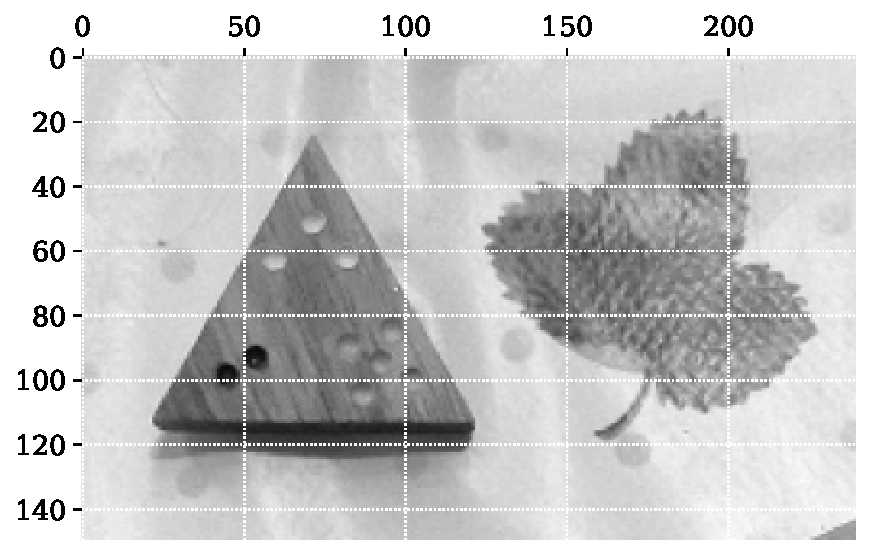
\includegraphics[width=.93\linewidth]{fragment_gray.pdf}
        \centering
        \caption{Одноканальное изображение}
        \label{fig:fragment_gray}
    \end{subfigure}
    \centering
    \caption{}
\end{figure}

На первом шаге мы переходим от трехканального изображения к одноканальному. По умолчанию программа оставляет только красный канал (\autoref{fig:fragment_gray}), поскольку стандартные формулы для перехода в оттенки серого в первую очередь учитывают зеленый, который в нашей задаче не дает хорошую отделимость. Далее в полученном изображении выделяются границы с помощью алгоритма Кэнни (\autoref{fig:fragment_canny}).

\begin{figure}[!h]
    \begin{subfigure}{.45\linewidth}
        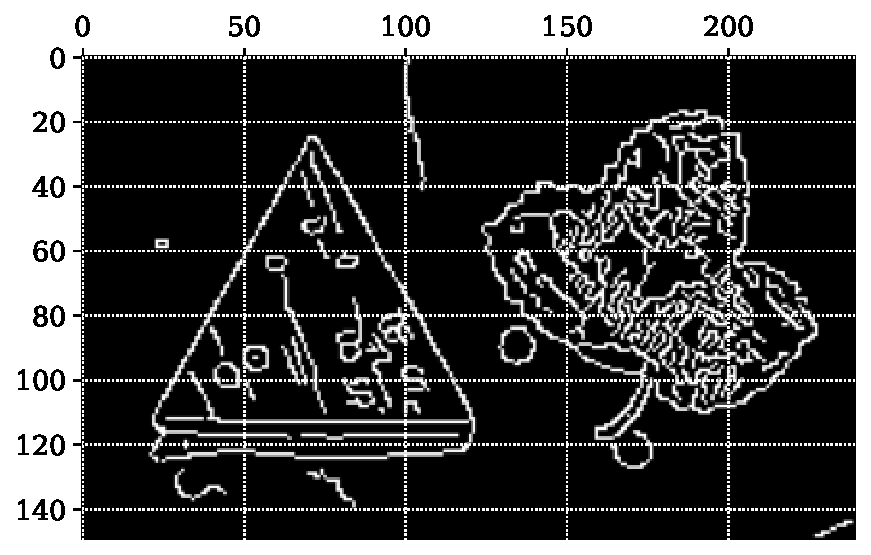
\includegraphics[width=.93\linewidth]{fragment_canny.pdf}
        \centering
        \caption{Оператор Кэнни}
        \label{fig:fragment_canny}
    \end{subfigure}
    \begin{subfigure}{.45\linewidth}
        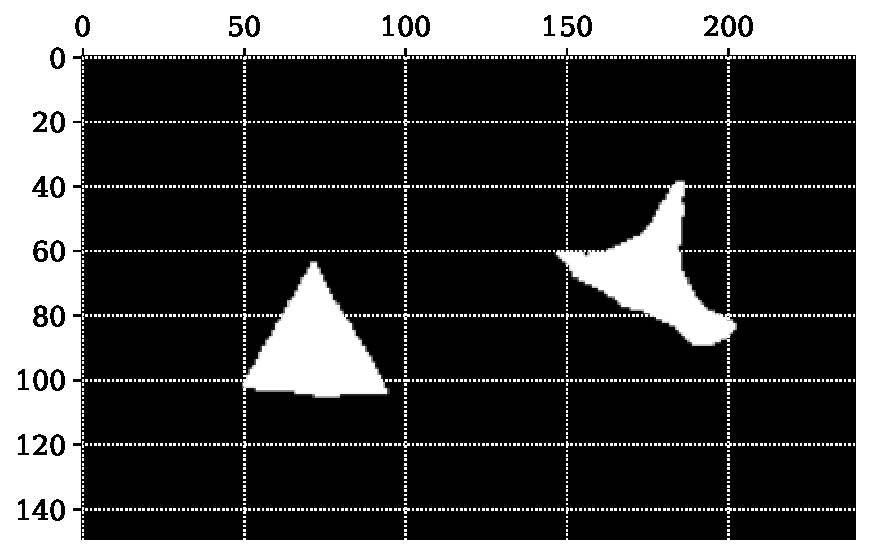
\includegraphics[width=.93\linewidth]{fragment_objects.pdf}
        \centering
        \caption{Морфологические операции}
        \label{fig:fragment_objects}
    \end{subfigure}
    \centering
    \caption{}
\end{figure}

Обнаружив границы, мы хотим избавиться от шума и всего, кроме треугольников. Применим последовательность морфологических операций: замыкание (чтобы обеспечить полный контур у всех треугольников), заполнение областей и достаточно агрессивная эрозия с кругом в качестве примитива. На выходе (\autoref{fig:fragment_objects}) мы получим заполненные, но уменьшенные треугольники, а также фоновые объекты, сравнимые по размеру с исходными фишками. Такая последовательность позволяет избавиться от большей части шума и сохранить форму треугольников.

\begin{figure}[!h]
    \begin{subfigure}{.45\linewidth}
        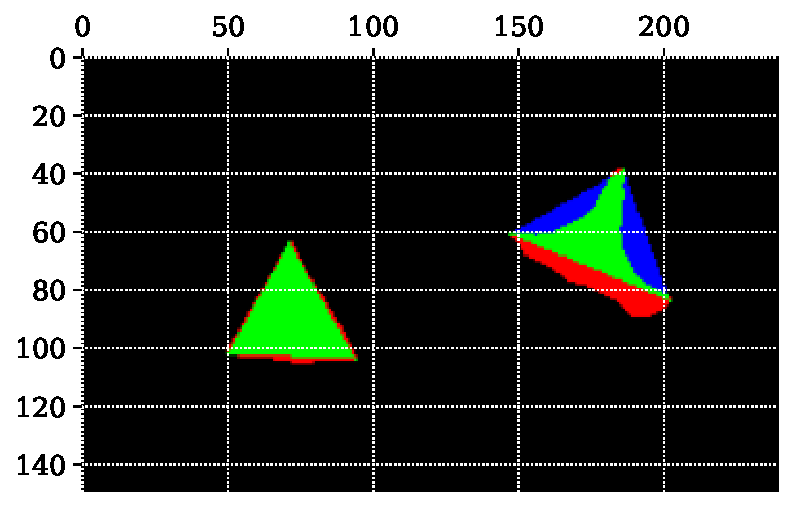
\includegraphics[width=.93\linewidth]{fragment_iou.pdf}
        \centering
        \caption{Иллюстрация IoU}
        \label{fig:fragment_iou}
    \end{subfigure}
    \begin{subfigure}{.45\linewidth}
        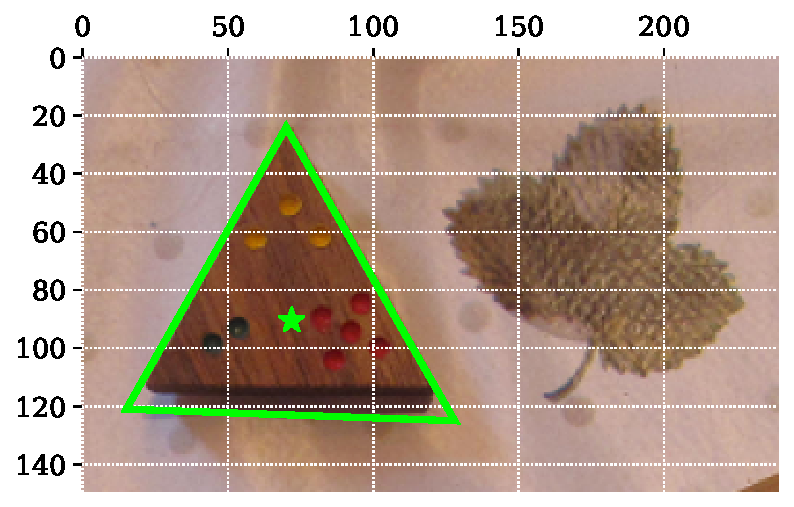
\includegraphics[width=.93\linewidth]{fragment_triangle.pdf}
        \centering
        \caption{Результат сегментации}
        \label{fig:fragment_triangle}
    \end{subfigure}
    \centering
    \caption{}
\end{figure}

Далее в каждом объекте (связной компоненте) ищутся 3 наиболее удаленных точки, максимизирующих периметр треугольника, который строится на этих вершинах. Но как понять, что мы действительно нашли фишку <<тримино>>? Для этого используется аналог коэффициента Жаккара для сегментации~--- IoU (Intersection over Union). В случае двух бинарных изображений эта величина численно равна площади пересечения (того, что мы считаем <<положительным>> классом, в данном случае белый цвет), разделенной на площадь объединения. С помощью IoU мы можем оценить, насколько построенный треугольник приближает исходную фигуру. Например, на \autoref{fig:fragment_iou} для левой компоненты $\text{IoU}\approx 0.88$, для правой~---$\text{IoU}\approx 0.43$. Оставляя только объекты с достаточно высоким IoU, мы получаем сегментированные фишки <<тримино>> с найденными вершинами и центром (\autoref{fig:fragment_triangle}). 

Осталось только посчитать число точек в углах найденных треугольников. Основная проблема данного этапа~--- разные цвета точек. Можно было бы использовать этот факт, например, находя хотя бы одну зеленую точку в окрестности угла, приписывать соответствующей вершине цифру <<2>>. Этот прием неплохо сработает на картинках с хорошим равномерным освещением, но в тривиальном варианте пригоден не для всех предложенных изображений.

\begin{figure}[!h]
    \begin{subfigure}{.45\linewidth}
        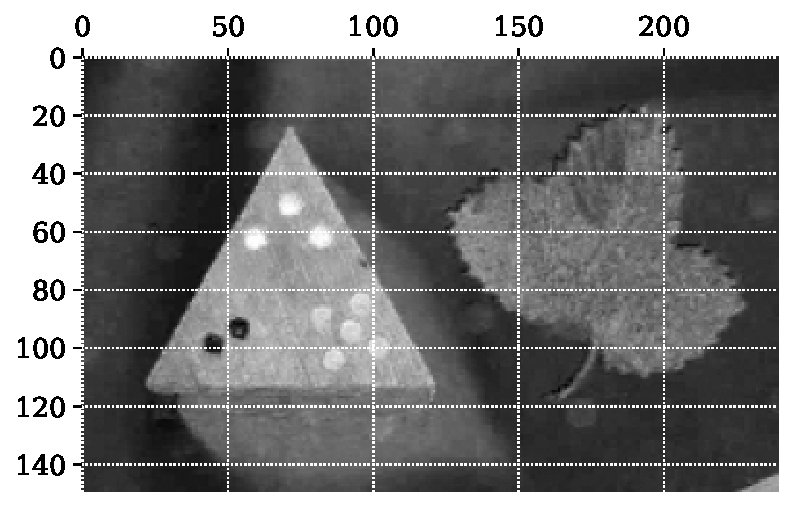
\includegraphics[width=.93\linewidth]{fragment_saturation.pdf}
        \centering
        \caption{Saturation}
        \label{fig:fragment_saturation}
    \end{subfigure}
    \begin{subfigure}{.45\linewidth}
        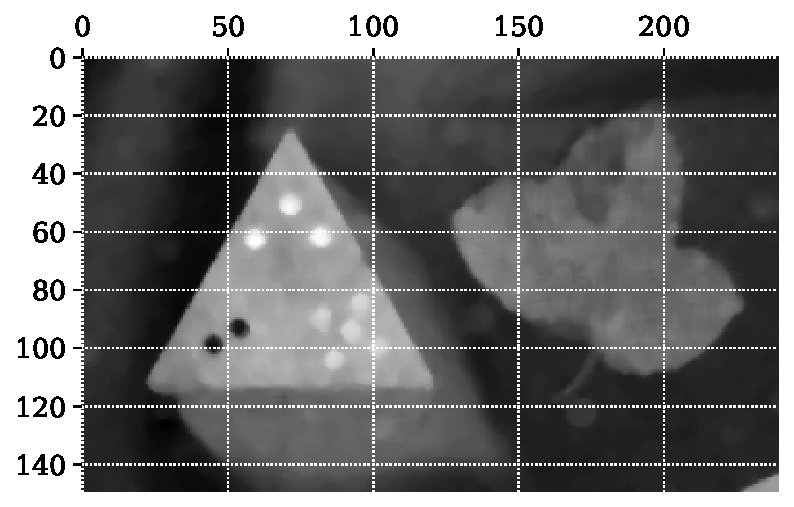
\includegraphics[width=.93\linewidth]{fragment_median.pdf}
        \centering
        \caption{Медианный фильтр}
        \label{fig:fragment_median}
    \end{subfigure}
    \centering
    \caption{}
\end{figure}

Будем бороться с неоднородными цветами другим способом. Для получения одноканального изображения на этом этапе посчитаем насыщенность (saturation) цвета. Сравнивая результат \autoref{fig:fragment_saturation} с \autoref{fig:fragment_gray}, замечаем, что такой подход позволяет хорошо выделять точки, цвет которых по сравнению с древесиной действительно более насыщенный.

Далее применим медианный фильтр (\autoref{fig:fragment_median}) и найдем границы с помощью алгоритма Кэнни (\autoref{fig:fragment_canny_2}). Причем используя маску сегментированных треугольников, мы можем оставить только то, что находится внутри. Чтобы отличить искомые точки от других элементов (границы фишки, текстуры древесины), мы воспользуемся морфологическими операциями, чтобы заполнить все небольшие полости. И именно заполненные связные компоненты небольшого размера будут соответствованить нужным точкам. Результат (центр масс каждого найденного объекта) приведен на \autoref{fig:fragment_dots}.

\begin{figure}[!h]
    \begin{subfigure}{.45\linewidth}
        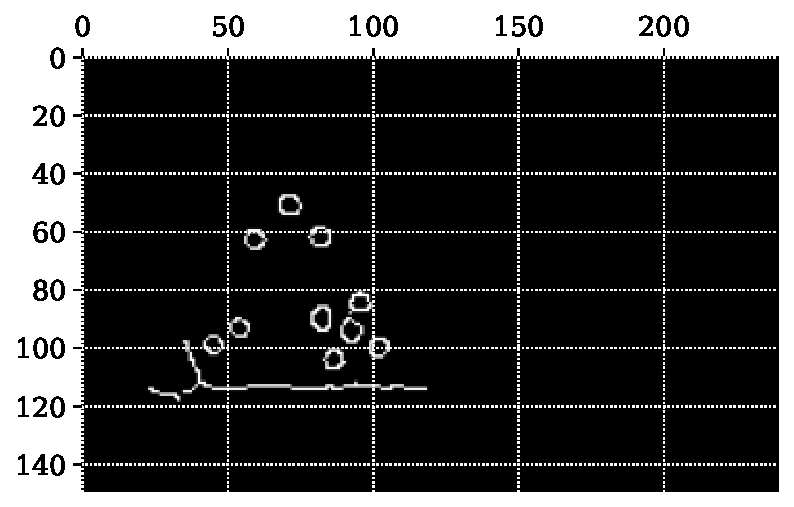
\includegraphics[width=.93\linewidth]{fragment_canny_2.pdf}
        \centering
        \caption{Оператор Кэнни}
        \label{fig:fragment_canny_2}
    \end{subfigure}
    \begin{subfigure}{.45\linewidth}
        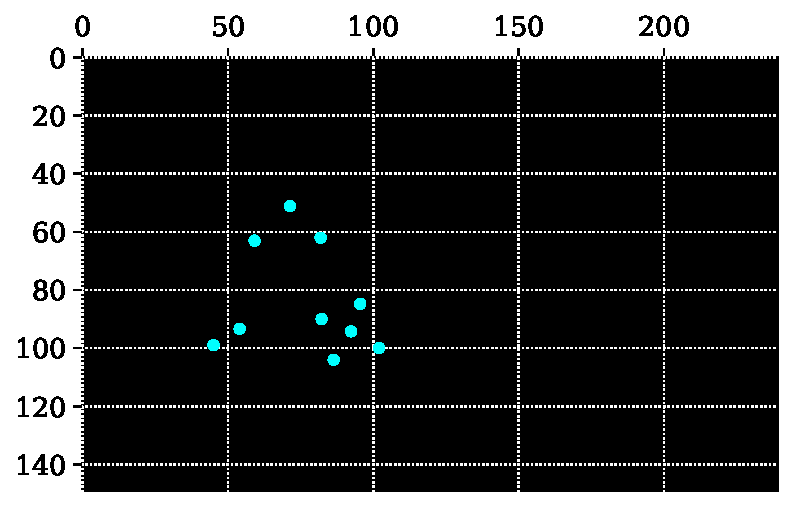
\includegraphics[width=.93\linewidth]{fragment_dots.pdf}
        \centering
        \caption{Найденные точки}
        \label{fig:fragment_dots}
    \end{subfigure}
    \centering
    \caption{}
\end{figure}

Остается только отнести точки к нужному углу. Для этого достаточно внутри каждого треугольника для каждой точки найти ближайшую вершину. Таким образом, мы находим все, что требуется в задании. Текстовый выход программы для этого небольшого фрагмента:
\begin{verbatim}
    1
    72, 91; 3, 2, 5
\end{verbatim}

Таким образом, мы можем эффективно сегментировать фишки <<тримино>> с помощью последовательности точечных, пространственных, алгебраических и морфологических операций.

\section{Программная реализация}
Для простого запуска программы в режиме <<черный ящик>> достаточно запустить скрипт \verb|trimino.py| с помощью команды
\begin{verbatim}
    python trimino.py input_image
\end{verbatim}
где \verb|input_image|~--- путь к входному изображению. Необходимые библиотеки будут приведены ниже. В процессе работы программа выведет на экран иллюстрацию сегментации и отметит найденные точки. Также иллюстрации будут сохранены в файле \verb|output_figure.png|, а требуемый формат вывода по заданию (число фишек, координаты центров, количество точек по углам)~--- в файле \verb|output.txt|. В процессе работы программа печатает в терминал текущий этап выполнения. Скриншот с примером работы приведен на \autoref{fig:screen}.

\begin{figure}[!h]
    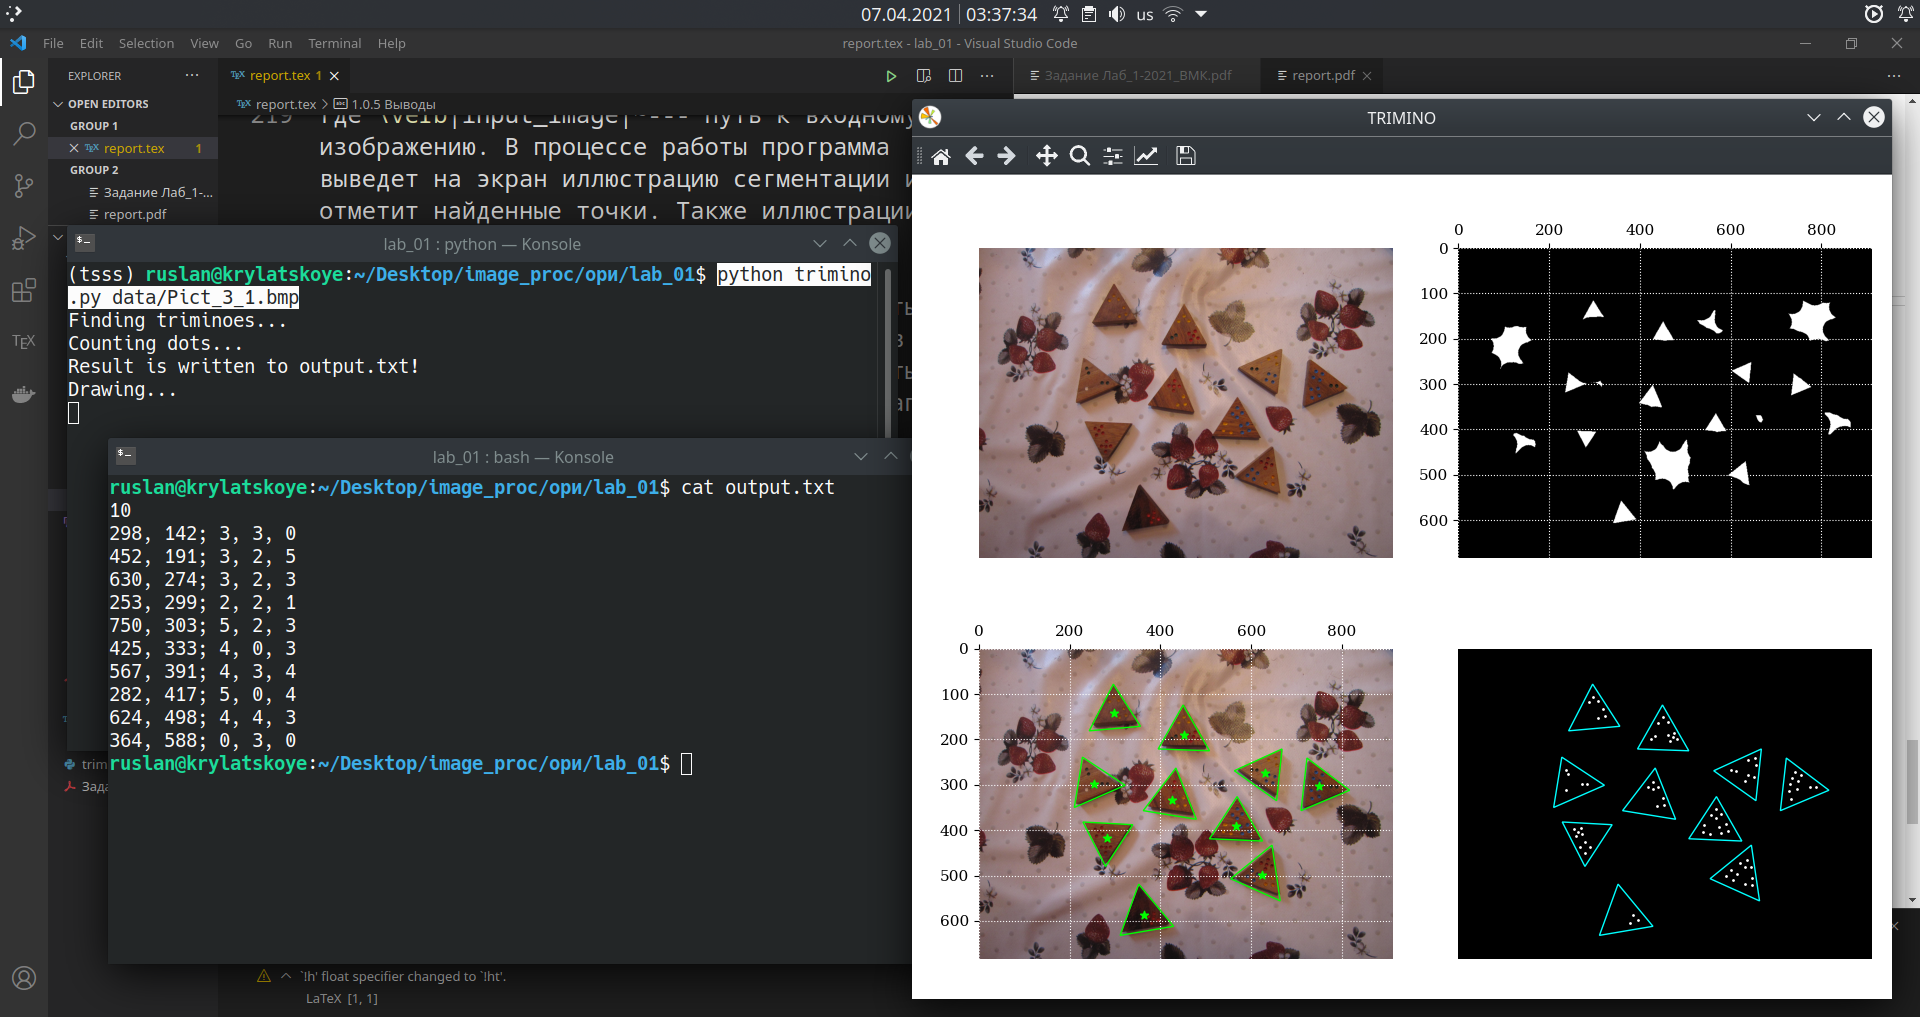
\includegraphics[width=\linewidth]{screenshot.png}
    \centering
    \caption{Скриншот, иллюстрирующий работу программы на изображении Pict\_3\_1}
    \label{fig:screen}
\end{figure}

Для более качественной работы возможно импротирование нужных функций из \verb|trimino.py|. Описанные в предыдущем разделе операции настраиваются: например, можно варьировать размеры структурообразующих элементов, параметры алгоритма Кэнни, выбирать метод перехода к одноканальному изображению и т.д.

Как уже ясно из способа запуска, программа написана на языке программирования Python с использованием библиотек:
\begin{itemize}
    \item \href{https://pypi.org/project/Pillow/}{pillow} для ввода-вывода изображений;
    \item \href{https://pypi.org/project/numpy/}{numpy} для векторных и матричных вычислений;
    \item \href{https://pypi.org/project/scikit-image/}{scikit-image} и \href{https://pypi.org/project/scikit-image/}{scipy.ndimage} для операций с изображениями;
    \item \href{https://pypi.org/project/matplotlib/}{matplotlib} для отрисовки графиков.
\end{itemize}

\section{Эксперименты}

Попробуем применить алгоритм к изображениям, приведенным на \autoref{fig:input}. На первом этапе (сегментация фишек) получим \autoref{fig:triple_segmantation}.

\begin{figure}[!h]
    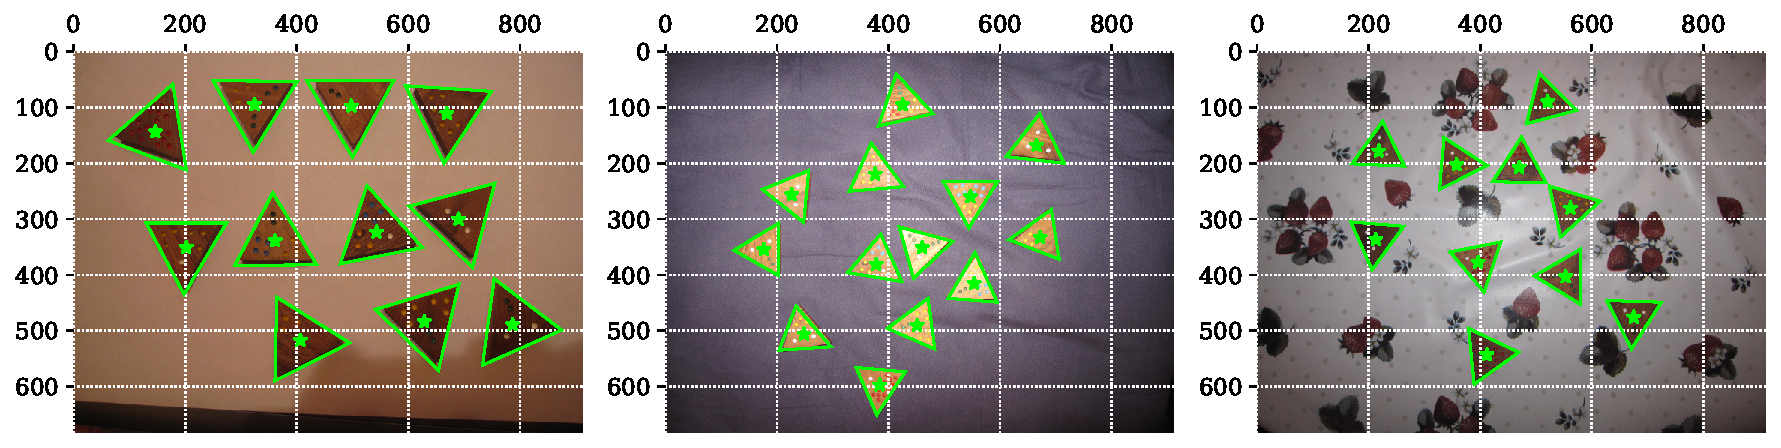
\includegraphics[width=\linewidth]{triple_segmantation.pdf}
    \centering
    \caption{Сегментация фишек <<тримино>>, три уровня сложности}
    \label{fig:triple_segmantation}
\end{figure}

Алгоритм с высокой точностью сегментирует треугольники. Теперь попробуем посчитать точки в углах фишек.

\begin{figure}[!h]
    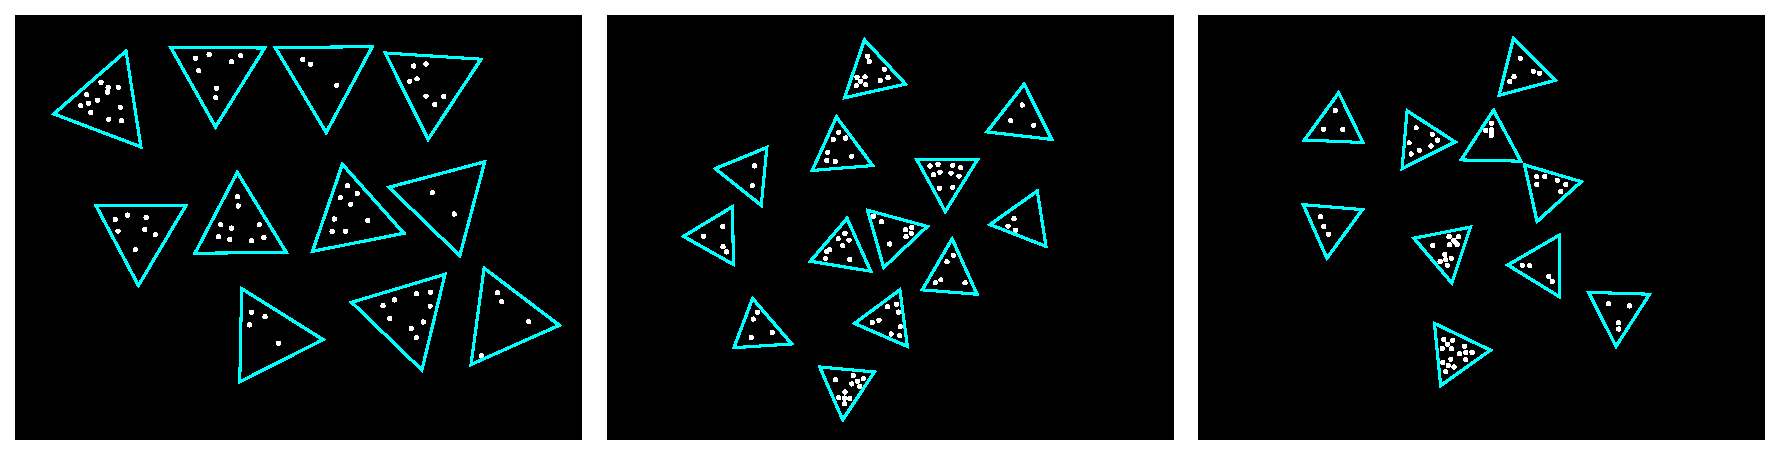
\includegraphics[width=\linewidth]{triple_dots.pdf}
    \centering
    \caption{Подсчет точек на обнаруженных фишках, три уровня сложности}
    \label{fig:triple_dots}
\end{figure}

Выделение точек \autoref{fig:triple_dots} оказалось более сложной задачей для программы: можно заметить, что точки обнаруживаются не со 100\%-й точностью.

Достаточно сложным элементом является <<5>>, состоящиая из красных точек. Из палитры фишек этот цвет наиболее близок к древесине, поэтому он и сливается. Интересно, в задаче обнаружения точек засвеченность фотографий помогает. Благодаря ярким бликам на <<Intermediate>> и <<Expert>> пятерки обнаруживаются лучше, чем на тусклом <<Beginner>>.

\section{Выводы}
Итак, по итогам данной лабораторной работы получена программа для сегментации фишем <<тримино>> и подсчета точек на них. Алгоритм, основанный на стандартных операциях с изоражениями, можно перенести на другие задачи сегментации примитивных форм. Отметим, что такой подход соответствует обучению без учителя: предоставленные изображения были использованы только для отладки и выбора гиперпараметров по умолчанию. Это определяет недостатки и преимущества метода: для качественной работы на новых данных может потребоваться заново настроить гиперпараметры, но отсутствие процедуры обучения делает использование алгоритма простым и быстрым.

\end{document}